\documentclass[a4paper,titlepage,10pt]{report}

\usepackage[T1]{fontenc}
\usepackage[utf8x]{inputenc}
\usepackage{polski}

\usepackage{enumerate}
\usepackage{amssymb}
\usepackage{amsmath}
\usepackage[pdftex]{graphicx}
\usepackage{tikz}
\usepackage[colorlinks=true,linkcolor=blue]{hyperref}
\usepackage{anysize}

\usepackage{lastpage}
\usepackage{fancyhdr}

\usepackage{subfig}

\usepackage{listings}

\lstset{numbers=left, stepnumber=1}
\usepackage[a4paper, top=2.5cm, bottom=2.5cm, left=2cm, right=2cm]{geometry}

\linespread{1.3}

%\title{\huge Symulacja układu planetarnego na GPU\\ przy użyciu CUDA i OpenGL\\\small Dokumentacja końcowa}
%\author{Daniel Kłobuszewski\and Jakub Kotur}
%\date{Promotor: Krzysztof Kaczmarski\\\vspace{24pt}\today}

\newcommand{\signature}[2]{
\begin{minipage}[]{#2}
\centering
\vspace{1.5em}
\rule{\linewidth}{0.5pt}
\vspace{0.5em}
#1
\end{minipage}
}

\begin{document}
	\thispagestyle{empty}
\begin{center}
\Large

\begin{minipage}{0.2\linewidth}
\centering

\includegraphics[height=2.86cm]{img/logo_pw.pdf}
\end{minipage}
\begin{minipage}{0.55\linewidth}
\centering
Politechnika Warszawska \\[0.5em] Wydział Matematyki \\ i Nauk Informacyjnych
\end{minipage}
\begin{minipage}{0.2\linewidth}
\centering

\includegraphics[height=2.86cm]{img/logo_mini.pdf}
\end{minipage}

\vspace{2em}
Praca dyplomowa inżynierska
\vspace{5em}

\huge
\textbf{Symulacja układu planetarnego na GPU przy użyciu CUDA i OpenGL}
%\\[0.5em] \textbf{English?}

\large

\vspace{4em}

\hfill
\begin{minipage}{0.4\linewidth}
Autorzy:
\vspace{0.5em}
\\
Daniel Kłobuszewski
\\
Jakub Kotur

\vspace{1em}

Promotor:
\vspace{0.5em}
\\
dr inż. Krzysztof Kaczmarski
\end{minipage}

\vfill
Warszawa, Styczeń 2011
\end{center}

	\newpage

	\tableofcontents
	\newpage

	\chapter{Wstęp}\label{chap:wstęp}
	\section{Streszczenie}\label{sec:streszczenie}
	\paragraph{}
Poniższy dokument stanowi podsumowanie projektu, pisanego w ramach przedmiotu Projekt Zespołowy, na wydziale Matematyki i Nauk Informacyjnych Politechniki Warszawskiej w semestrze zimowym 2010/2011.

\paragraph{}
Opisujemy w nim zasady działania głównych modułów, różnice w stosunku do specyfikacji oraz wnioski z testów akceptacyjnych. Znajduje się tutaj także krótka instrukcja obsługi programu, która pozwoli zapoznać się z nim każdej osobie, która wcześniej nie miała z naszą aplikacją styczności.

	\newpage
	\section{Podstawy teoretyczne}\label{sec:podstawy teoretyczne}
	\subsection{Deferred rendering}\label{sub:deferred rendering}
\paragraph{}

Silnik graficzny został napisany przy użyciu popularnej ostatnio techniki deferred rendering~\cite{gpugems:deferred}~\cite{calver:deferred}. Jest ona popularna dopiero od niedawana, ponieważ wymaga stosunkowo nowych i silnych kart graficznych. Pozwala jednak na dużą kontrolę nad procesem renderowania oraz umożliwia tworzenie ciekawych efektów graficznych w stosunkowo łatwy sposób. Bardzo dobrze sprawdza się również przy dużej ilości obiektów oraz otwartych przestrzeniach. Nadaje się zatem idealnie do wyświetlania układów planetarnych. Wybór tej techniki pozwolił także na optymalizację, dzięki której geometria w programie została ograniczona do niezbędnego minimum. Spowodowało to pewne dodatkowe koszty, jednak były one o wiele niższe niż w przypadku standardowego podejścia forward renderingu.

\paragraph{}

Deferred rendering polega na dwuprzejściowym generowaniu finalnego obrazu. W pierwszym przejściu, przeliczana jest geometria, a wynik tych obliczeń wpisywany jest do specjalnego bufora geometrii, nazywanego g-buforem. W g-buforze zapisywane są informacje o pozycji, normalnej oraz kolorze danego piksela ekranu. W zależności od danego silnika bufor ten może zawierać różne dane. W drugim przejściu, na podstawie tego bufora liczone są wszystkie efekty graficzne, takie jak oświetlenie, cienie, dla każdego piksela oddzielnie. Takie podejście pozwala na bardzo wiele oraz jest stosunkowo wydajne, posiada jednak wady. Poniżej przedstawione są wady jak i zalety deferred renderingu.

\paragraph{Zalety}

\begin{description}
\item{Skalowalność} - ponieważ ciężkie obliczenia liczone są dla piksela, silnik ten doskonale skaluje się zarówno ze względu na dodawanie geometrii do sceny, jak i na oddalanie i zbliżanie kamery do obiektów na scenie

\item{Duża kontrola} - dzięki jawnemu tworzeniu buforów ekranu, można stworzyć wiele niestandardowych efektów graficznych

\end{description}

\paragraph{Wady}

\begin{description}
\item{Wielkość buforów} - bufory ekranu zajmują bardzo dużo miejsca, przy rozdzielczości full hd może być to nawet 50MB, co dla starych kart graficznych było wielkościami ogromnymi
\item{Przezroczystość} - ponieważ obliczenia są robione tylko raz dla każdego piksela ekranu, niemożliwe jest zrobienie przezroczystości w ten sposób
\item{Dużo obliczeń} - niezależnie od sceny obliczenia są proporcjonalne do wielkości ekranu i robione dla piksela. Dla starych kart graficznych jest to o wiele za ciężkie rozwiązanie
\item{Wymagane MRT} - ponieważ buforów jest wiele, wymagana od karty jest technologia MRT, czyli multiple render target, dzięki której można wygenerować jednocześnie wszystkie bufory. Na starych kartach graficznych potrzebne było tyle przejść ile jest buforów, co powoduje wielokrotne obliczenia geometrii
\end{description}

\subsection{Układy planetarne i klasteryzacja}\label{sub:uklady planetarne}

\paragraph{}
Zadanie silnika fizycznego w najprostszym ujęciu nie jest zbyt skomplikowane. Musi on na bieżąco obliczać położenia planet, podczas gdy oddziałują na nie pozostałe planety. Zasadniczo złożoność takich obliczeń jest rzędu \ensuremath{O(n^2)} w każdej klatce fizyki. Siła oddziaływania planet między sobą jest opisana znanym z liceum wzorem:

		$$ \overrightarrow{F_{ij}} = G\frac{m_i m_j}{r^2}\overrightarrow{e_{ij}}  $$

gdzie: 

$ \overrightarrow{F_{ij}} $ - wektor siły działającej na ciało $i$ w wyniku oddziaływania z ciałem $j$. 

$ G $ - stała grawitacji. 
 
$ m_i $ - masa ciała $i$. 

$ r $ - odległość ciał $i$ oraz $j$. 

$ e_{ij} $ - wektor jednostkowy, skierowany od ciała $i$ do ciała $j$. 

\paragraph{}

Jak widać z powyższego wzoru, siła maleje wprost proporcjonalnie do $ \frac {1}{r^2} $. W praktyce oznacza to, że dla pojedynczych, odległych od siebie planet, siła oddziaływania jest pomijalnie niska. W związku z tym można podzielić przestrzeń na klastry, wewnątrz których liczone są wszystkie oddziaływania. Ponadto, liczone są także sumaryczne oddziaływania klastrów między sobą, a prędkość wypadkowa z tych oddziaływań jest dodawana do prędkości każdej z planet w klastrze.

\paragraph{}
Rozważmy złożoność obliczeniową jednej klatki fizyki przy podziale przestrzeni na klastry. Zakładamy, że $n$ planet podzielono na $k$ klastrów, przy czym każdy klaster zawiera $\frac{n}{k}$ planet. Ilość oddziaływań wewnątrz wszystkich klastrów wynosi:
$$ k\left(\frac{n}{k}\right)^2 = \frac{n^2}{k}$$

\paragraph{}
Należy także obliczyć oddziaływania pomiędzy całymi klastrami planet. Wyliczenie środków oraz sumarycznych mas klastrów wymaga
$$ k\frac{n}{k} = n $$

\paragraph{}
obliczeń. Oddziaływań klastrów między sobą jest natomiast
$$ k^2 $$

\paragraph{}
Po zsumowaniu otrzymujemy faktyczną złożoność algorytmu:
$$ O( \frac{n^2}{k} + n + k^2 ) = O( \frac{n^2}{k} + k^2 ) $$

W efekcie, jeżeli przyjmiemy liczbę klastrów równą $\sqrt[3]{n^2}$, złożoność wyniesie $O(n\sqrt[3]{n})$. W praktyce okazuje się, że jest to zbyt duża wartość. Wynika to m.in. z faktu, iż podział na klastry zwykle nie jest równomierny. Należy także pamiętać o narzucie obliczeniowym związanym z wyliczaniem samych klastrów, który został w powyższym rozumowaniu pominięty.

\paragraph{}
Do podziału przestrzeni planet na klastry używany jest algorytm k-means\cite{kmeans}. Jest to algorytm heurystyczny, przez co trudno jest szacować jego złożoność. W ogólnym przypadku problem klasteryzacji jest problemem NP-trudnym. Wynik oraz czas działania algorytmu k-means zależą znacząco od wyboru punktów początkowych. W naszym przypadku idealnymi punktami początkowymi są środki $k$ najcięższych planet, gdyż skupiają one wokół siebie inne, lżejsze ciała. Pozwala to na zadowalająco szybkie znajdowanie poprawnych klastrów przy użyciu tego algorytmu.


	\chapter{Instrukcja}\label{chap:instrukcja}
	\section{Instrukcja instalacji}\label{sec:instrukcja użytkownika}
	\subsection{Wymagania}\label{sub:wymagania}
\paragraph{}

Aplikacja została napisana z użyciem takich technologii jak CUDA i OpenGL. Implikuje to dość spore wymagania co do karty graficznej wymaganej do uruchomienia programu. Ponieważ użyliśmy wyżej wymienione komponenty w wersjach, CUDA 2.3 oraz OpenGL 3.2, karta graficzna musi być co najmniej NVIDIA geForce serii 8, lub nowsza. Jednak aby móc uruchomić program z pełnymi możliwościami graficznymi, oraz dla dużych układów planet zalecana jest karta serii 200, lub któraś z mocniejszych kart serii 9.

\paragraph{}





	\section{Instrukcja użytkownika}\label{sec:instrukcja użytkownika}
	%\subsection{Opcje startowe}\label{sub:uruchamianie programu}
%\paragraph{}

\subsection{Poruszanie kamerą}\label{sub:poruszanie kamerą}
\paragraph{}
Kamera w aplikacji jest swobodna, co oznacza, że możemy poruszać i obracać nią we wszystkich kierunkach. Do przesuwania kamery w przód i w tył służą odpowiednio klawisze W i S. Przesunięcia w lewo i w prawo odbywają się przy pomocy klawiszy A i D, natomiast ruch w górę i w dół jest możliwy przy użyciu klawiszy Q i E. Tę ostatnią czynność możemy zrealizować także korzystając z klawisza Ctrl i spacji.
\paragraph{}
Do wykonywania obrotów należy użyć myszy. Jest ona używana także do korzystania z GUI. Do odróżnienia tych dwu czynności używany jest prawy przycisk myszy. Kiedy jest on wciśnięty, ruchy myszką odpowiadają "rozglądaniu się" w przestrzeni kosmicznej. 
\paragraph{}
Dodatkowo, jeżeli chcemy śledzić jakąś planetę, a nie chce nam się ciągle lecieć za nią kamerą, wystarczy, że klikniemy na nią lewym klawiszem myszy. Wówczas kamera automatycznie będzie zmieniała swoje położenie tak, aby nie zmieniać odległości od zaznaczonej planety. W takim trybie można dalej swobodnie się rozglądać, ale już nie poruszać. Aby wrócić do swobodnego trybu kamery, wystarczy kliknąć gdzieś w przestrzeń kosmiczną.

\subsection{Interfejs graficzny}\label{sub:interfejs graficzny}
\paragraph{}

Po uruchomieniu aplikacji pokazuje się okno przedstawiające kosmos. Na nim znajdują się również guziki. Przy ich pomocy możliwe jest wczytanie bądź zapisanie układu planet. Można również wystartować lub zatrzymać animację. Dostępne są też różne opcje programu, takie jak modyfikacji szybkości kamery, szybkości animacji oraz inne opcje graficzne i fizyczne. W tym rozdziale przedstawione będzie użycie podstawowych możliwości GUI. Dla oszczędności tuszu, kolory na obrazkach są odwrócone w porównaniu do oryginalnej aplikacji.

\begin{figure}[ht!]
\centering
\fbox{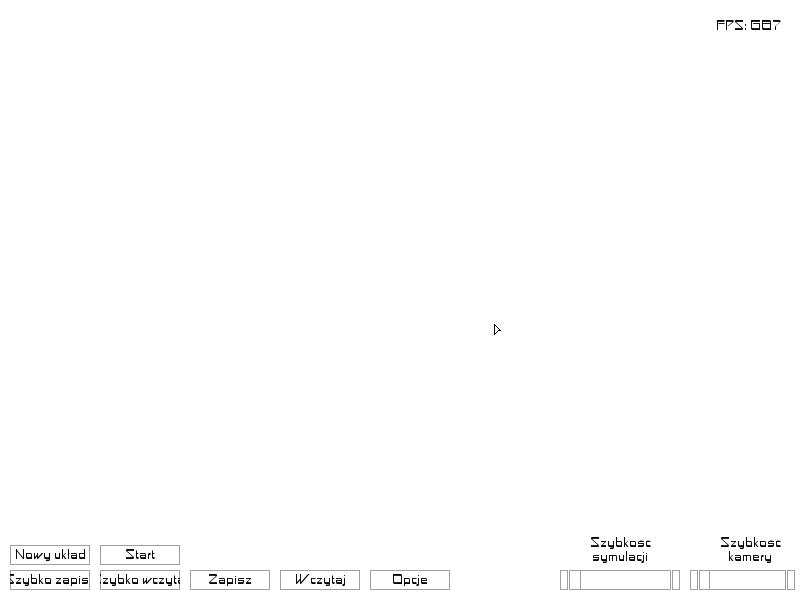
\includegraphics[width=0.75\textwidth]{img/inst_00.png}}
\caption{Początkowe okno}
\label{fig:inst_00}
\end{figure}

\subsubsection{Odczyt}\label{ssub:odczyt}
\paragraph{}

Po wciśnięciu guzika wczytaj, na ekranie pojawi się okno wczytywania. Możemy na nim wybrać interesujący nas układ. Po wybraniu układu oraz wciśnięciu "Wczytaj" układ zostanie załadowany. Można również wcisnąć guzik "Szybko wczytaj" który pozwoli na natychmiastowe wczytanie układu o nazwie "qsave.sav".

\begin{figure}[ht!]
\centering
\fbox{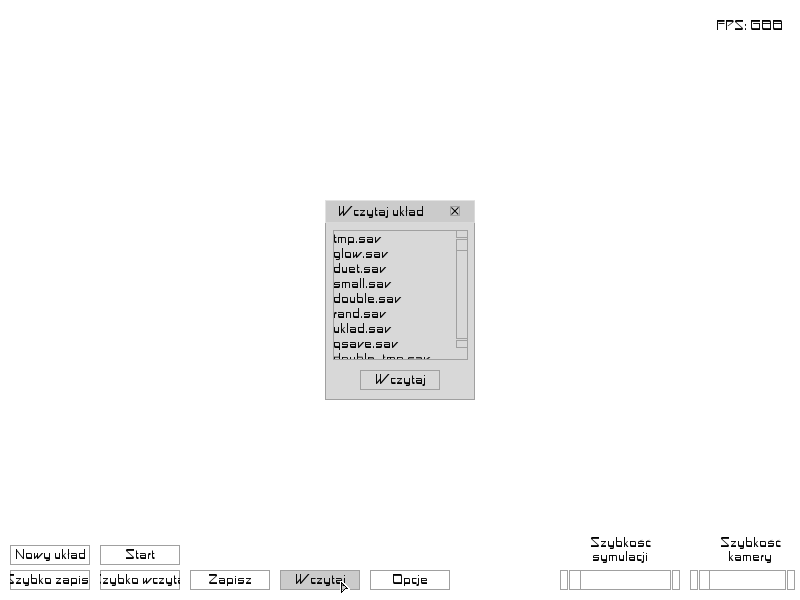
\includegraphics[width=0.75\textwidth]{img/inst_06.png}}
\caption{Okno wczytywania}
\label{fig:inst_01}
\end{figure}

\begin{figure}[ht!]
\centering
\fbox{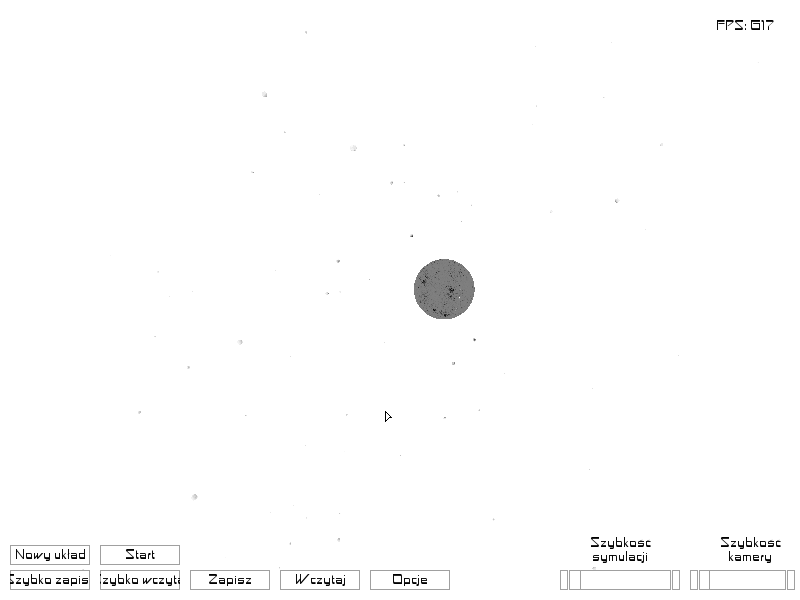
\includegraphics[width=0.75\textwidth]{img/inst_02.png}}
\caption{Wczytany układ}
\label{fig:inst_02}
\end{figure}

\subsubsection{Start animacji}\label{ssub:start animacji}
\paragraph{}

Układ domyślnie wczytywany jest w trybie pauzy. Aby wystartować animację należy wcisnąć guzik start. Powinien on w tedy zmienić nazwę i funkcję na puaza, a planety powinny zacząć się poruszać.

%\begin{figure}[ht!]
%\centering
%\fbox{\includegraphics[width=0.75\textwidth]{img/inst_03.png}}
%\caption{Animacja}
%\label{fig:inst_03}
%\end{figure}

\subsubsection{Zapis układu}\label{ssub:zapis ukladu}
\paragraph{}

Jeżeli aktualny stan układu się nam podoba, możemy go zapisać. Należy w tym celu wcisnąć guzik "Zapisz", po wciśnięciu którego na ekranie pojawi się okno. W oknie tym należy wpisać nazwę nowego układu, oraz wcisnąć guzik "Zapisz" na oknie. Od tej pory nowy układ będzie dostępny do wczytania przez aplikację.


\begin{figure}[ht!]
\centering
\fbox{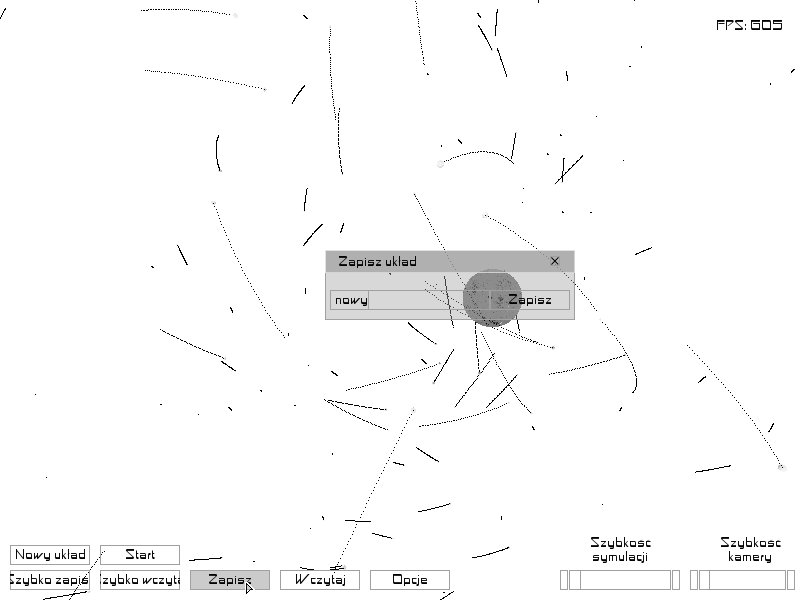
\includegraphics[width=0.75\textwidth]{img/inst_07.png}}
\caption{Okno zapisu}
\label{fig:inst_04}
\end{figure}

\subsubsection{Opcje}\label{ssub:opcje}
\paragraph{}

Na głównym ekranie znajdują się również dwa suwaki, którymi można zmieniać odpowiednio prędkość symulacji, oraz szybkość kamery. Pierwszy suwak odpowiada za liczbę klatek fizyki na jedną klatkę programu. Drugi natomiast zmienia szybkość poruszania kamery w przestrzeni. Dodatkowo po wciśnięciu guzika "Opcje" który znajduje się w głównym ekranie aplikacji, jest dostęp do dodatkowych opcji programu. Można tam manipulować ustawieniami graficznymi, fizycznymi i innymi.



	\chapter{Projekt}\label{chap:projekt}
	\section{Przypadki użycia}\label{sec:przypadki użycia}
	\section{Przypadki uzycia}\label{sec:usecase}

\paragraph{}

Poniższy diagram przedstawia przypadki użycia aplikacji przez użytkownika. Ponieważ najważniejszym elementem aplikacji są obliczenia na karcie graficznej, oraz wyświetlanie ich wyników w przyjaznej dla oka formie, główną aktywnością użytkownika jest oglądanie efektów obliczeń i cieszenie oka efektami specjalnymi. Jednak aby aplikacja była choć trochę funkcjonalna, użytkownikowi umożliwione będzie podstawowa kontrola symulacji.

\begin{figure}[h]
	\centering
	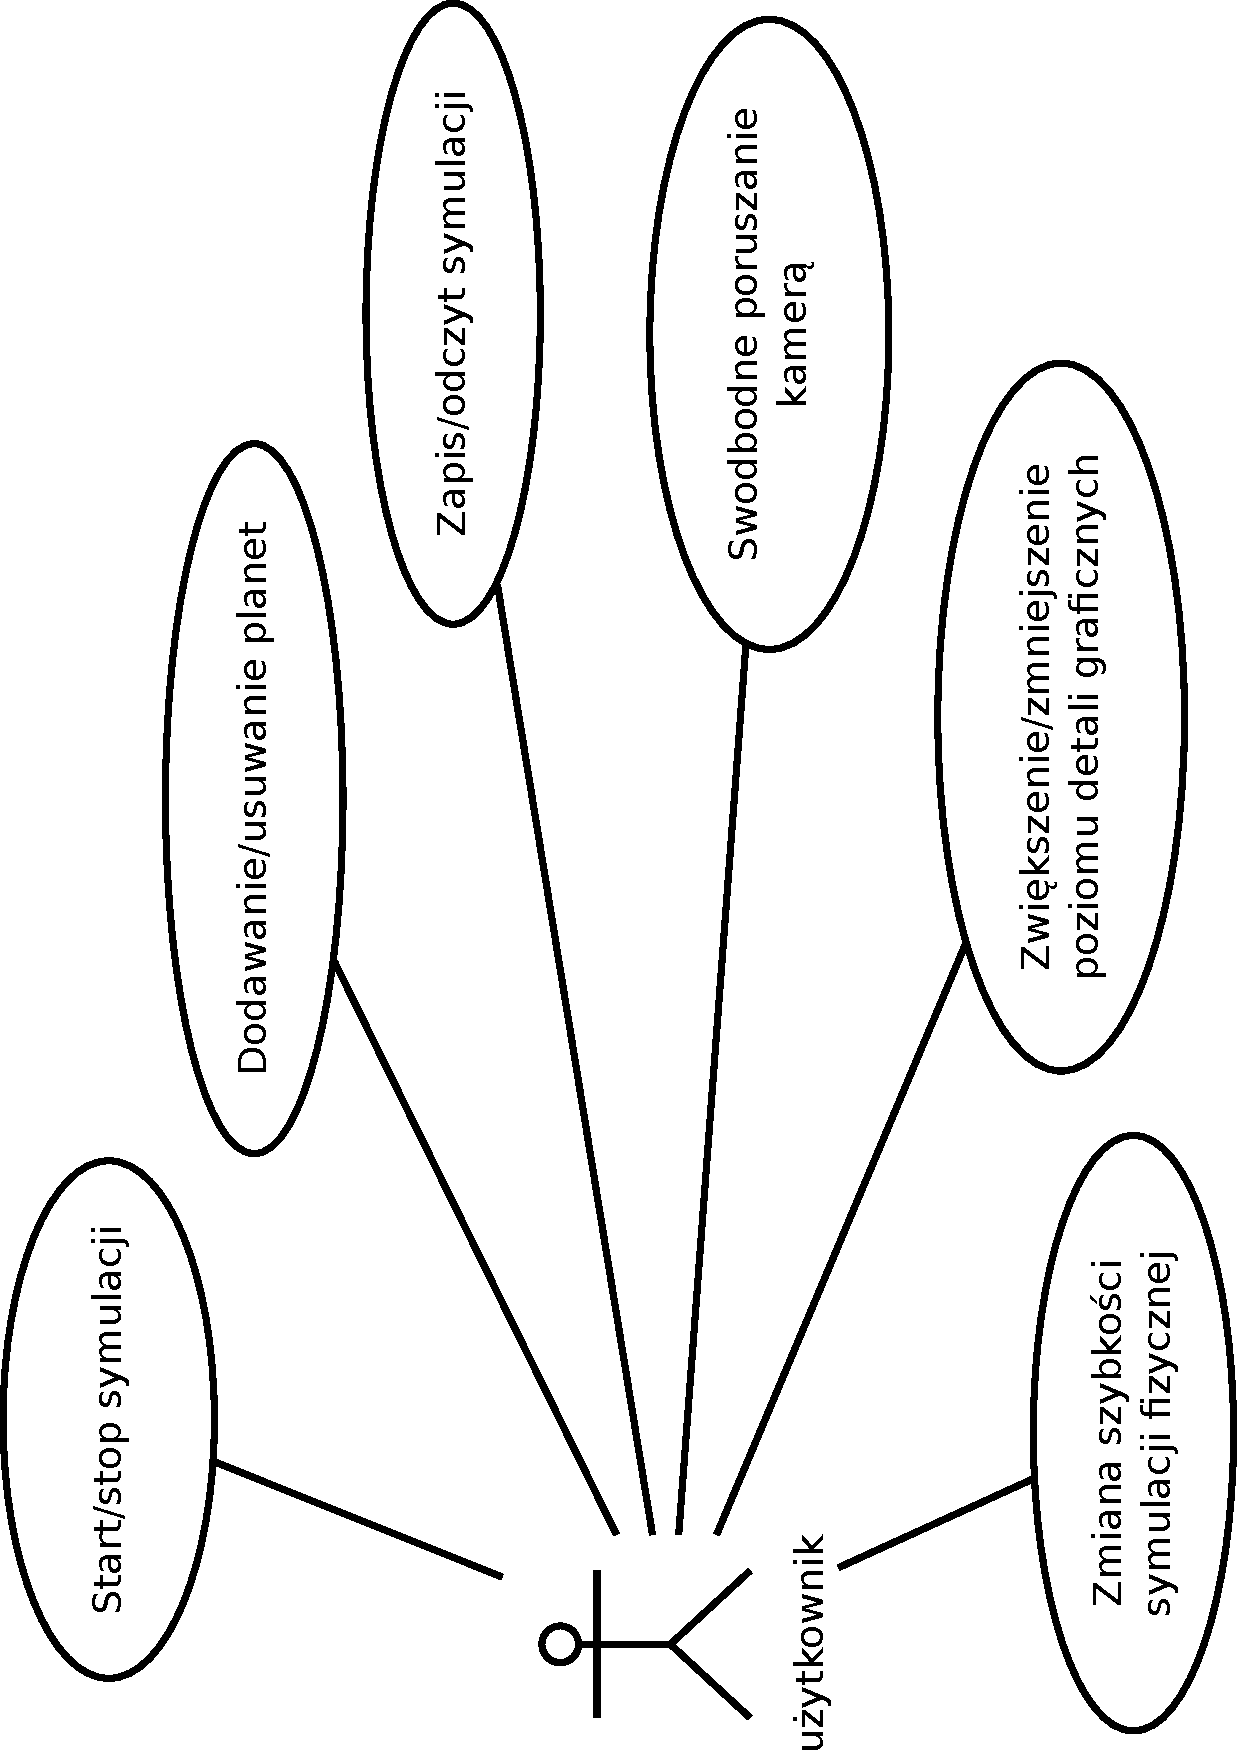
\includegraphics[width=0.5\textwidth,angle=-90]{use-case.pdf}
	\caption{Diagram przypadków użycia}
	\label{fig:use-case}
\end{figure}

\paragraph{}

Znaczenie poszczególnych przypadków użycia dla aplikacji jest następujące:

\begin{description}
	\item[Start/stop symulacji] - aplikacja powinna przewidywać możliwość zatrzymania i wznowienia symulacji fizycznej, nie blokując przy tym możliwości poruszania kamera. W trybie pauzy powinna być również możliwość dodawania/usuwania planet.
	\item[Dodawanie/usuwanie planet] - aby dać użytkownikowi możliwość budowania własnych układów, aplikacja powinna pozwalać na usuwanie planet uczestniczących w aktualnej symulacji, oraz na dodawanie nowych planet, nadając im masę, pozycje, oraz prędkość początkowa. Wygodnym sposobem ustawiania nowej planety jest używanie myszki, dla ustalenia pozycji, oraz prędkości początkowej.
	\item[Zapis/odczyt symulacji] - aplikacja powinna pozwalać na wczytywanie wcześniej zdefiniowanych układów, ponieważ uzyskanie stabilnego układu planetarnego nie jest rzeczą prostą. Jeśli jednak sie to uda, powinna być również możliwość zapisania aktualnego stanu symulacji.
	\item[Swobodne poruszanie kamera] - swobodna kamera oznacza, ze można przesuwać ja w dowolnym kierunku, tak aby była możliwość ustawienia jej w dowolnej pozycji, oraz można ja obracać w dowolna stronę. Na przesuwnie kamery najwygodniej pozwolić za pomocą klawiszy klawiatury, natomiast obroty najwygodniej realizuje sie poprzez ruch myszki.
	\item[Zmiana poziomu detali graficznych] - w zależności od mocy karty graficznej na maszynie wywołującej program, powinna być możliwość ustawienia szczegółowości prezentowanej symulacji. Miedzy innymi można sterować ilością wierzchołków składających sie na obiekt (teselacja), rozdzielczością oraz sposobem mapowania tekstur, ilością prezentowanych efektów specjalnych, ilością gwiazd (źródeł światła).
	\item[Zmiana szybkości symulacji fizycznej] - w zależności od możliwości jednostki graficznej na której dokonywane są obliczenia fizyczne, można ustawić więcej, bądź mniej klatek fizycznych na jedna klatkę graficzna, tak aby uzyskać tak samo dokładną symulacje w krótszym czasie.
\end{description}


	\section{Architektura}\label{sec:architektura}
	\subsection{Działanie programu}\label{sub:dzialanie programu}
\paragraph{}

Podstawowymi aktywnościami projektu są moduły wyświetlania planet oraz obliczania pozycji planet. Jednak dla działania aplikacji bardzo ważne są również inne aktywności, które mimo, że prostsze w implementacji mają duży wpływ na architekturę projektu. Poniższy diagram przedstawia kolejne aktywności aplikacji podczas działania. Dodatkowo na diagramie przedstawiony jest przepływ najważniejszych informacji, czyli pozycji planet.

\paragraph{}

\begin{figure}[ht!]
	\centering
	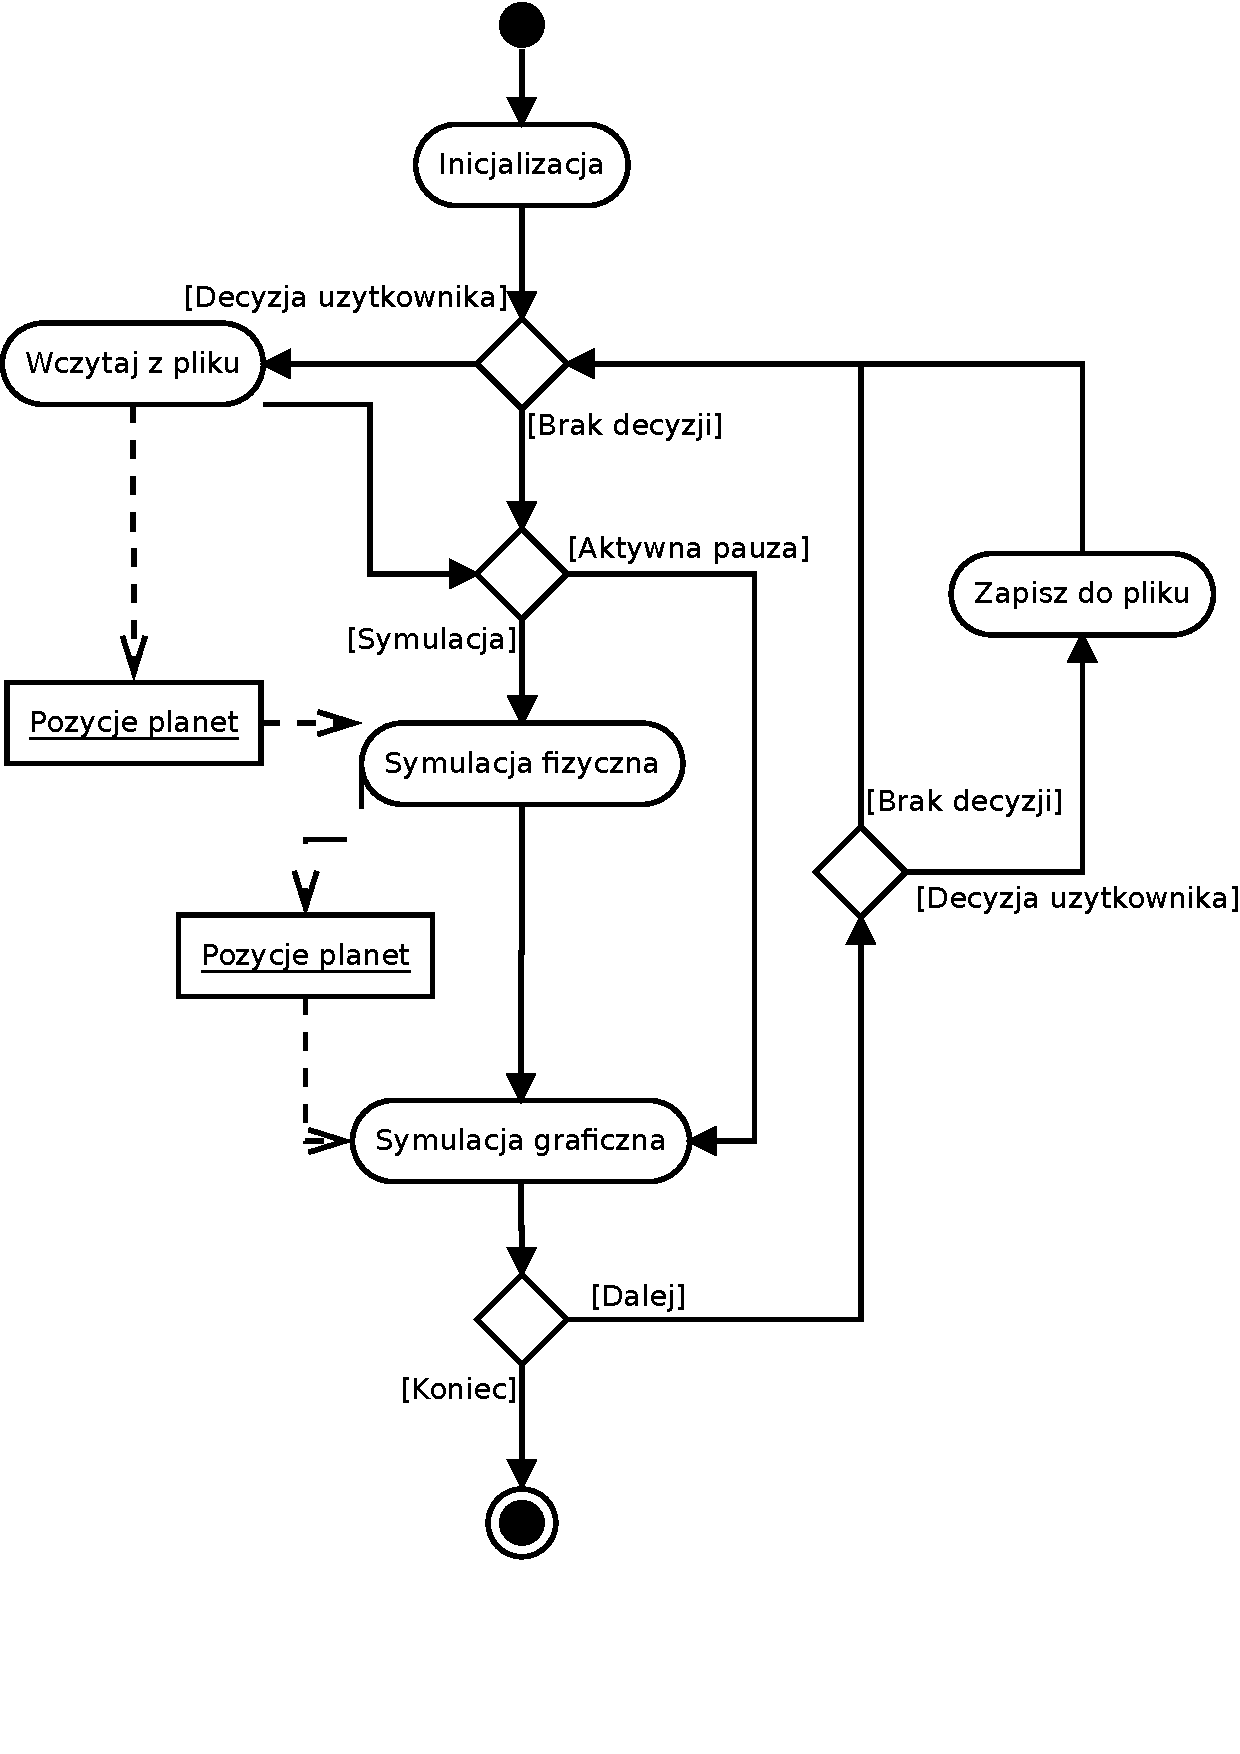
\includegraphics[width=0.75\textwidth]{activity.pdf}
	\caption{Diagram aktywności}
	\label{fig:activity}
\end{figure}


\begin{description}
	\item[Inicjalizacja aplikacji] \hfill \\
	Jest to pierwsza aktywność jaką wykonuje program. Składa się ona z inicjalizacji wszystkich modułów, w szczególności modułu graficznego i fizycznego. Zajmuje się także początkową alokacją pamięci i wczytaniem wszystkich potrzebnych zasobów, takich jak tekstury, modele oraz inne potrzebne dane.
	\item[Wczytanie z pliku] \hfill \\
	Jeśli użytkownik zdecyduje zacząć symulację z wcześniej przygotowanego pliku ta akcja jest za to odpowiedzialna. Musi ona załadować potrzebne dane z pliku oraz zapisać je poprzez pamięć RAM jednostki głównej do pamięci RAM jednostki graficznej. Użytkownik może również zdecydować o wczytaniu z pliku podczas już trwającej symulacji. W takim przypadku konieczne jest również zadbanie o odpowiednie wyczyszczenie poprzedniej symulacji, tak aby żadne artefakty nie zostały w pamięci RAM, zarówno jednostki głównej, jak i graficznej.
	\item[Zapis do pliku] \hfill \\
	Na życzenie użytkownika aktualny stan symulacji może zostać zapisany do pliku. W takim przypadku zbierane z aplikacji są wszystkie potrzebne dane, takie jak pozycje planet, wielkości i ciężary planet, modele planet, pozycja kamery itp. oraz zapisywane są do pliku.
	\item[Aktywna pauza] \hfill \\
	Symulacja wspiera tak zwaną "aktywną pauzę". Oznacza to, że na żądanie użytkownika symulacja fizyczna jest zatrzymana, natomiast cały czas reszta aplikacji jest w pełni funkcjonalna. Oznacza to, że można sterować kamerą, wczytywać/zapisywać układy planetarne oraz dodawać/usuwać planety.
	\item[Symulacja fizyczna] \hfill \\
	Jest to kluczowy moduł dla działania aplikacji. Podczas każdej takiej aktywności obliczane są kolejne pozycje planet do wyświetlenia. W jednej iteracji może być obliczona więcej niż jedna klatka fizyczna, jeśli moc obliczeniowa komputera na to pozwala.
	\item[Symulacja graficzna] \hfill \\
	Ta aktywność odpowiedzialna jest przede wszystkim za wyświetlanie symulacji na ekranie. Głównym jej zadaniem jest wyświetlanie planet na ich pozycjach wraz z towarzyszącymi im efektami graficznymi. Pozycje planet do wyświetlenia pobierane są z modułu fizycznego. Jeśli natomiast włączona jest aktywna pauza i nowe pozycje nie zostały wygenerowane, moduł korzysta ze starych pozycji. Po zakończonej jednej iteracji pętli, aplikacja odczekuje chwilę, żeby nie zajmować całego procesora oraz żeby zapewnić takie samo działanie symulacji na słabszych komputerach (gdzie czekanie może zostać pominięte)
\end{description}

\subsection{Struktura klas}\label{sub:struktura klas}
\paragraph{}
Ze względu na architekturę aplikacji, klasy używane na CPU oddzielone są od klas karty graficznej. Oczywiście te drugie są klasami jedynie logicznie - ze względu na konieczność używania języka C w kodzie dla GPU. Jednak ze względu na to, że obiekty są wygodną abstrakcją, będziemy z niej korzystać w całym programie.

\subsubsection{Klasy GPU}

\begin{figure}[h]
	\centering
	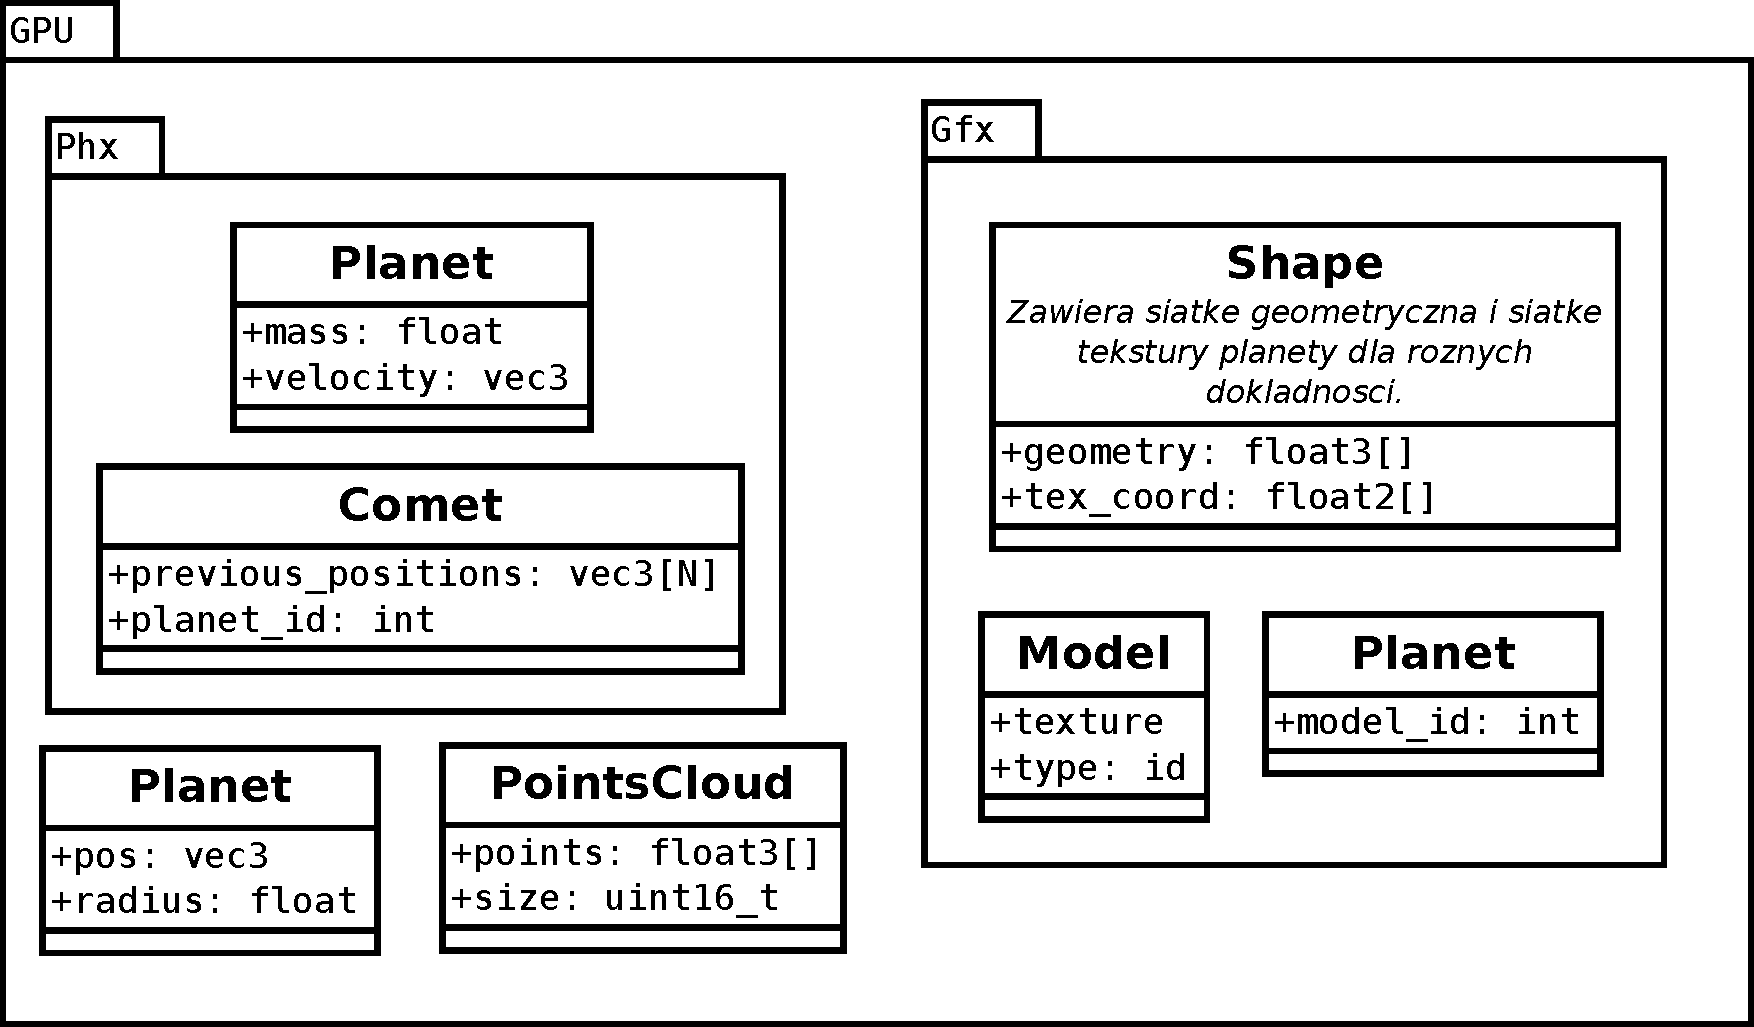
\includegraphics[angle=0,width=0.8\textwidth]{img/class_gpu.pdf}
	\caption{Diagram klas dla GPU}
	\label{fig:class_gpu}
\end{figure}

\paragraph{}
Struktury, z których będziemy korzystać na karcie graficznej, określone są na rysunku \ref{fig:class_gpu}. Ponieważ karta graficzna służy nam zarówno do wyświetlania danych, jak i do ich przetwarzania, wydzielone są na nim dwie przestrzenie nazw. Są to:
\begin{itemize}
	\item{Phx - do operacji fizycznych}
	\item{Gfx - do operacji graficznych}
\end{itemize}

\paragraph{}
Ponadto istnieje kilka struktur wspólnych dla obu częsci.

\begin{description}
\item[\texttt{ GPU::Planet}] zawiera informacje, z których korzystają zarówno wyświetlanie jak i fizyka. Jest to położenie planety oraz jej promień.
\item[\texttt{ GPU::PointsCloud}] reprezentuje chmurę cząstek - jest ona obliczana dla każdej widocznej komety przez moduł fizyczny.
\end{description}

\paragraph{}

Operacje fizyczne odbywać się będą z wykorzystaniem dwóch dodatkowych struktur.

\begin{description}
\item[\texttt{ GPU::Phx::Planet}] to dodatkowe informacje o każdej planecie, które są potrzebne jedynie silnikowi fizycznemu. Należą do nich prędkość oraz masa.
\item[\texttt{ GPU::Phx::Comet}] stanowi dodatkową informację o planecie. Struktura ta istnieje tylko dla obiektów będących kometami. Zawiera kilka ostatnich pozycji oraz identyfikator planety.
\end{description}

\paragraph{}

Do wyświetlenia planet konieczne będą informacje o teksturach oraz o siatkach każdej z planet.

\begin{description}
\item[\texttt{ GPU::Gfx::Planet}] zawiera indeks modelu, czyli wyglądu planetu. Dwie planety mogą mieć ten sam model.
\item[\texttt{ GPU::Gfx::Model}] definiuje konkretny wygląd. Na tym poziomie będziemy rozróżniać zwykłe planety od gwiazd i komet.
\item[\texttt{ GPU::Gfx::Shape}] agreguje informację o siatce planety w 3D oraz odpowiadającej jej siatce na dwuwymiarowej teksturze.
\end{description}

\subsubsection{Klasy CPU}

\begin{figure}[ht!]
	\centering
	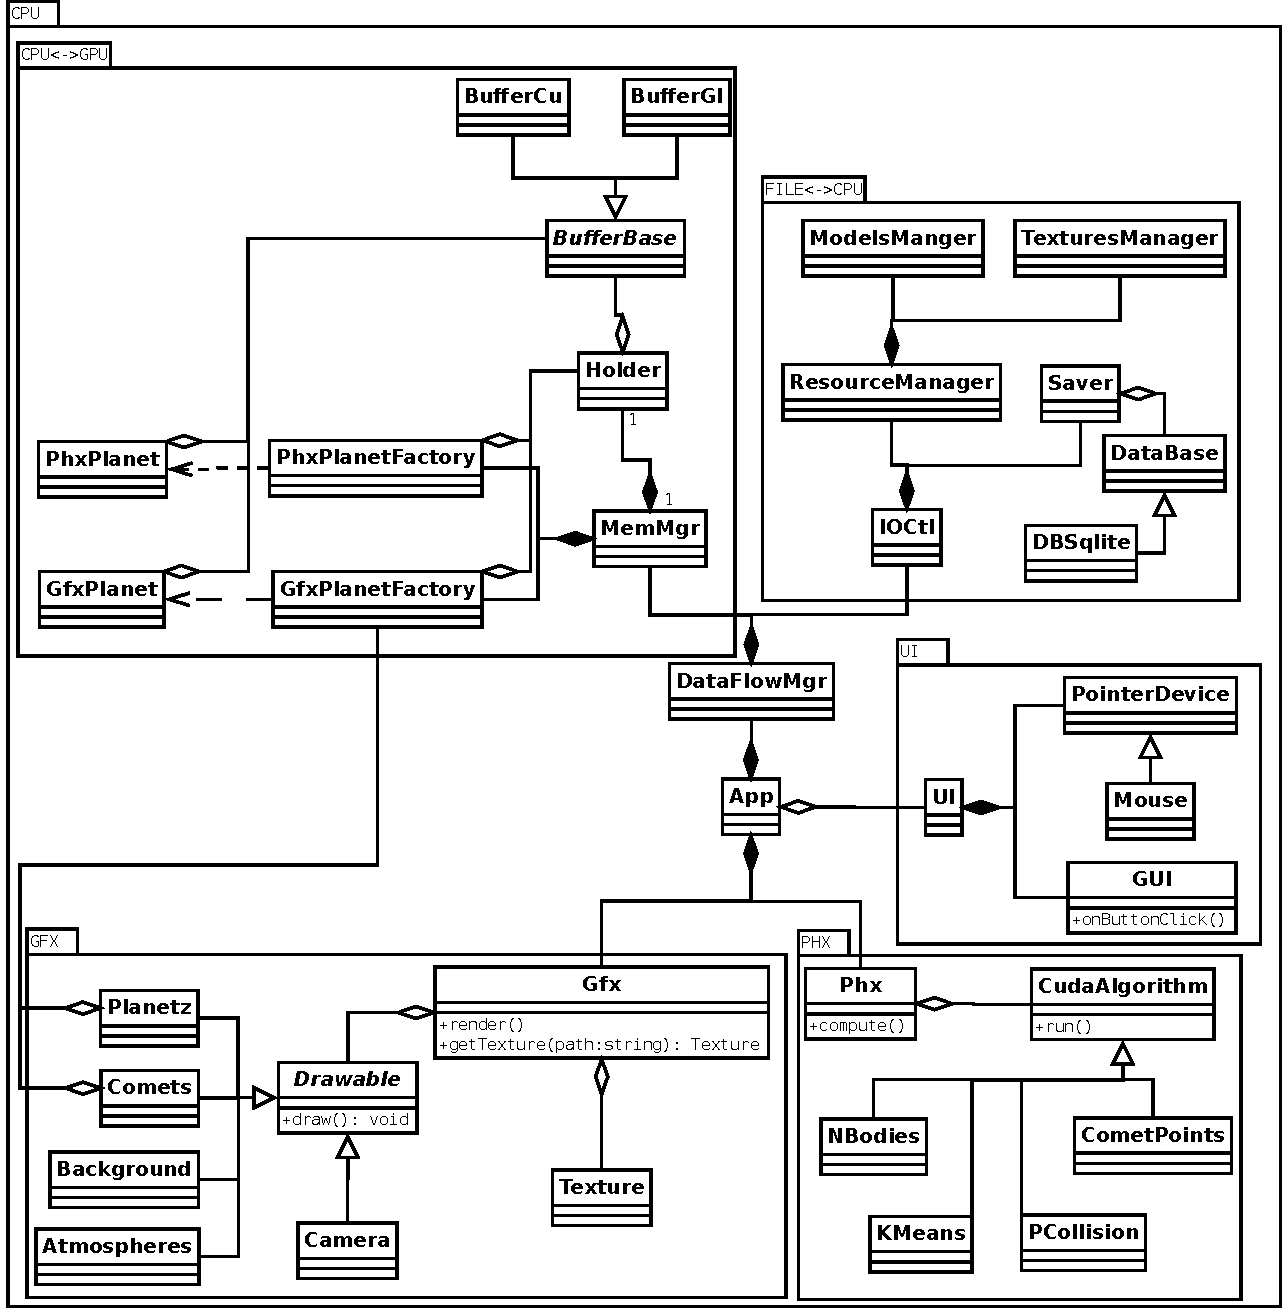
\includegraphics[angle=0,width=\textwidth]{img/class_cpu.pdf}
	\caption{Diagram klas dla CPU}
	\label{fig:class_cpu}
\end{figure}

\paragraph{}
Ta część klas przełoży się bezpośrednio na klasy znane z c++. Diagram klas znajduje się na rysunku \ref{fig:class_cpu}.

\begin{description}
\item[\texttt{ CPU::App}] jest główną klasą, zarządzającą obiektami GFX, PHX, DataFlowMgr oraz UI. Tworzy je ona na początku działania programu.
\item[\texttt{ CPU::DataFlowMgr}] wykonuje wszystkie przepływy danych - pomiędzy RAM karty graficznej, RAM komputera oraz dyskiem twardym.
\item[]
\item[\texttt{ CPU::PHX::Phx}] zarządza wykonaniem algorytmów wykonywanych na karcie graficznej.
\item[\texttt{ CPU::PHX::CudaAlgorithm}] abstrakcyjna klasa reprezentująca algorytm karty graficznej. Jeden algorytm może składać się z wywołań kilku kerneli CUDA.
\item[\texttt{ CPU::PHX::NBodies}] podstawowy algorytm w projekcie - wyliczenie oddziaływań planet między sobą.
\item[\texttt{ CPU::PHX::KMeans}] algorytm liczenia klastrów. W wersji podstawowej - standardowy algorytm k-means.
\item[\texttt{ CPU::PHX::PCollision}] algorytm wykrywający kolizje między planetami. W wersji podstawowej - uwzględnia jedynie kolizje wewnątrz klastrów.
\item[\texttt{ CPU::PHX::CometPoints}] obliczenie chmury punktów, służących do wyświetlenia ogona komety.
\item[]
\item[\texttt{ CPU::GFX::Gfx}] odpowiada za wyświetlanie wszystkich obiektów obecnych w przestrzeni 3D. Korzysta przy tym z biblioteki OpenGL.
\item[\texttt{ CPU::GFX::Drawable}] abstrakcja dla wszystkich obiektów, które chcą być wyświetlane.
\item[\texttt{ CPU::GFX::Texture}] obiekt tekstury, generowany przez klasę Gfx na podstawie bitmapy. Można zapobiec zbędnemu ładowaniu tekstur. Każda klasa, aby dostać taki obiekt, musi poprosić o niego klasę Gfx, która albo zwróci załadowaną teksturę, albo stworzy nowy obiekt tej klasy.
\item[\texttt{ CPU::GFX::Planetz}] obiekt wyświetlający wszystkie planety obecne na scenie.
\item[\texttt{ CPU::GFX::Comets}] obiekt wyświetlający wszystkie komety.
\item[\texttt{ CPU::GFX::Background}] wyświetla tło.
\item[\texttt{ CPU::GFX::Atmospheres}] klasa odpowiedzialna za wyświetlanie efektów atmosferycznych nad planetami.
\item[]
\item[\texttt{ CPU::UI::UI}] odpowiada za całość interakcji z użytkownikiem, czyli za obsługę zdarzeń myszki, klawiatury oraz graficzny interfejs użytkownika.
\item[\texttt{ CPU::UI::GUI}], czyli graficzny interfejs użytkownika. Składać sie na to będą okna oraz guziki zagnieżdżone w oknie głównym aplikacji.
\item[\texttt{ CPU::UI::PointerDevice}] abstrakcja dla wszystkich wejściowych urządzeń, które mogą być wskaźnikami. W danej aplikacji będzie to najprawdopodobniej myszka, jednak takie podejście umożliwia dodanie obsługi takich peryferii jak dżojstiki czy kontrolery gier.
\item[\texttt{ CPU::UI::Mouse}] implementacja abstrakcji wskaźnika z użyciem myszki.
\item[]
\item[\texttt{ CPU::FILE2CPU::IOCtl}] klasa bazowa modułu odpowiedzialnego za wczytywanie danych z plików do pamięci ram oraz zapisywanie zmodyfikowanych danych do pliku.
\item[\texttt{ CPU::FILE2CPU::ResourcesManager}] klasa odpowiedzialna za zarządzenie zasobami aplikacji, takimi jak modele, tekstury i wszelkie inne dane przechowywane na dysku.
\item[\texttt{ CPU::FILE2CPU::ModelsManager}] służy do wczytywania modeli planet z dysku do pamięci RAM.
\item[\texttt{ CPU::FILE2CPU::TexturesManager}] służy do wczytywania tekstur do bitmap w pamięci RAM.
\item[\texttt{ CPU::FILE2CPU::DataBase}] abstrakcyjna klasa służąca do komunikacji aplikacji z bazą danych. Aplikacja będzie najprawdopodobniej korzystać z bazy sqlite, która jest idealna do takich zastosowań, jednak użycie abstrakcji pozwoli na bezbolesną podmianę bazy w razie konieczności.
\item[\texttt{ CPU::FILE2CPU::DBSqlite}] implementacja abstrakcji bazy danych do komunikacji z bazą sqlite.
\item[]
\item[\texttt{ CPU::CPU2GPU::MemMgr}] na zlecenie DataFlowMgr'a przenosi dane pomiędzy kartą graficzną a RAM.
\item[\texttt{ CPU::CPU2GPU::Holder}] Agreguje wszystkie bufory potrzebne do reprezentacji planety. Zarówno te fizyczne, graficzne, jak i wspólne.
\item[\texttt{ CPU::CPU2GPU::BufferBase}] bazowa, abstrakcyjna klasa dla buforów jednostki graficznej. Dzięki temu danymi dostępnymi dla programów jednostki graficznej można wygodnie manipulować z poziomu kodu jednostki centralnej.
\item[\texttt{ CPU::CPU2GPU::BufferCu}] reprezentuje dane przetrzymywane na karcie graficznej przy pomocy wywołań biblioteki CUDA.
\item[\texttt{ CPU::CPU2GPU::BufferGl}] reprezentuje dane przetrzymywane na karcie graficznej przy pomocy wywołań biblioteki OpenGL. Technologia CUDA pozwala na udostępnianie buforów opengla dla programów CUDA, dzięki temu bufor ten używany jest tam, gdzie potrzebny jest dostęp do danych zarówno z modułów graficznych, jak i fizycznych.
\item[\texttt{ CPU::CPU2GPU::PhxPlanetFactory}] jest faktorią dla obiektów reprezentujących planety z punktu widzenia fizyki na karcie graficznej.
\item[\texttt{ CPU::CPU2GPU::GfxPlanetFactory}] analogiczna klasa, ale tworząca obiekty graficzne.
\item[\texttt{ CPU::CPU2GPU::PhxPlanet}] obiekt zawierający bufory karty graficznej potrzebne do obliczeń fizycznych.
\item[\texttt{ CPU::CPU2GPU::GfxPlanet}] analogiczny do PhxPlanet, z tą różnicą, że posiada niemodyfikowalne bufory potrzebne do wyświetlania planet.
\end{description}



	\chapter{Opis działania}\label{chap:opis dzialania}
	\section{Silnik graficzny}\label{sec:silnik graficzny}
	
\subsection{Konstrukcja silnika}\label{sub:konstrukcja silnika}
\paragraph{}

Silnik jest silnikiem wielo-przejściowym. Dla wyświetlenia planet wraz z oświetleniem i teksturami, potrzebne są dwa przejścia. Jedno do wygenerowania g-bufora, drugie do wygenerowania końcowego obrazu. Ponieważ w tym podejściu niemożliwe jest uzyskani przezroczystości, aby wyświetlić półprzezroczyste atmosfery konieczne jest wyświetlenie ich oddzielnie. Są one tak samo jak planety wyświetlanie dwoma przejściami przy użyciu deferred renderingu. Cały silnik posiada więc cztery przejścia, po dwa dla obrazów planet i atmosfer. Następnie wyniki tych przejść są nakładane na siebie z uwzględnieniem przezroczystości.

\subsection{Dane pośrednie}\label{sub:dane pośrednie}
\paragraph{}

Silnik graficzny potrzebuje dużego bufora pośrednich danych. Buforem tym z uwagi na wygodę używania jest dwuwymiarowa tekstura zmiennoprzecinkowa. 

\subsection{Generowanie geometrii}\label{sub:generowanie geometrii}
\paragraph{}

Dzięki zastosowaniu deferred renderingu, oraz tego, że renderowanymi obiektami są jedynie kule, można ominąć standardowy proces generowania geometrii. Kula która daje zadowalający efekt i jest wyświetlana przy pomocy zestawu wierzchołków, musiała by ich mieć około tysiąca. Samo przetwarzanie takiej geometrii jest kosztowne, dodatkowo doszły do tego ograniczenia karty graficznej i geometry shaderów, które trzeba by obchodzić, narażając się na dodatkowe koszty.

\paragraph{}

Wiedząc że jedyne obiekty które chcemy wyświetlić są kulami, wiemy że obiekt taki z każdej strony wygląda tak samo. Jesteśmy również w stanie łatwo policzyć składową z kuli, mając jedynie koordynaty w osiach OX i OY na tej kuli. Dzięki tym spostrzeżeniom, można stworzyć mapę głębokości (koordynat na osi OZ) kuli. Dzięki takiej mapie, w pierwszym przebiegu, wyświetlane są jedynie płaskie kwadraty, które dzięki mapie głębokości, są w stanie do bufora ekranu przekazać poprawną informację o pozycji piksela w przestrzeni. Dodatkowo ta sama mapa stanowi mapę normalnych dla oświetlenia. Dzięki takiemu podejściu, każda planeta generuje jedynie cztery wierzchołki, a reszta geometrii jest odczytywana z tekstury.

\paragraph{}

Niestety tak pięknie by to wyglądało, gdyby zastosowany był rzut ortogonalny. W symulacjach jednak konieczne do zastosowania jest rzut projekcyjny. W takim przypadku planeta widoczna na krawędzi kamery, różni się od planety widocznej na wprost. W skrajnym przypadku, gdy widoczne jest 360°, możemy widzieć planetę zupełnie od tyłu. Dlatego konieczne są dodatkowe obliczenia, uwzględniające położenie planety względem kamery.

\subsection{Obliczanie oświetlenia}\label{sub:obliczanie oświetlenia}
\paragraph{}

Obliczanie oświetlenia na podstawie buforów ekranów nie stanowi problemu. W programie zastosowane jest model oświetlenia Phonga, natomiast obliczenia prowadzone są dla każdego piksela oddzielnie. Dodatkowo w celach optymalizacyjnych, nie jest liczone światło odbite (specular), ponieważ planety mają powierzchnię chropowatą, więc i tak oświetlenie to by miało znikomy wpływ na efekt końcowy, natomiast jest dość kosztowne obliczeniowo.

\paragraph{}

W celu optymalizacji, dodatkowo do każdej gwiazdy (źródła światła) przypisany jest jej zakres świecenia. Dzięki temu oświetlenie z gwiazd, które nie oświetlają planet odległych od siebie, nie jest obliczane. W przypadku gwiazd nie jest to tak znaczna optymalizacja jak w przypadku bardzo słabych świateł, jak na przykład lampki choinkowe, jednak sprawdza się przy kilku odległych od siebie galaktykach.

\subsection{Nakładanie tekstur}\label{sub:nakladanie tekstur}
\paragraph{}

Skomplikowaniu ze względu na użycie deferred renderingu uległo niestety nakładanie tekstur na planety. Tekstura, tak samo jak wspomniana wcześniej mapa normalnych, jest nakładana na kulę w zależności od koordynat na osiach OX i OY. Jednak w odróżnieniu od mapy normalnych, tekstura zależy od obrotu kamery względem planety, i z każdej strony wygląda inaczej. Pojawiły się więc dwa problemy. Obracanie koordynat tekstury, tak aby widz miał wrażenie że planeta faktycznie się obraca, oraz mapowanie koordynat kwadratu reprezentującego planetę, na koordynaty tekstury planety.

\paragraph{}

Pierwszy problem został rozwiązany poprzez przekazywanie obrotu kamery do silnika graficznego, poprzez przekazanie macierzy obrotu kamery. Następnie uzyskane koordynaty kuli, są przemnażane przez tą macierz. W ten sposób otrzymywany jest bezwzględna pozycja kuli, na którą patrzy aktualnie kamera.

\paragraph{}

Drugim problemem jest mapowanie tekstury na kulę, tak aby z koordynat kuli 3D, uzyskać koordynaty na teksturze 2D. W standardowym podejściu, stosuje się siatki tekstury, natomiast każdy trójkąt jest interpolowany na płaszczyźnie. W naszym podejściu nie ma trójkątów, trzeba więc było uzyskać ciągły sposób mapowania, bez żadnych siatek. Z pomocą przyszła kartografia, która zna liczne sposoby mapowania płaszczyzny na kulę i z powrotem. Najlepsze okazały się metody mapowania o stałej powierzchni. Oznacza to że parametrem który nie ulega zniekształceniu ze względu na położenie na kuli, jest powierzchnia. Dzięki temu po mapowaniu tekstury na kulę, zniekształcenia są najmniejsze. Najtańszą obliczeniowo z tych metod okazała się metoda sinusoidalna, która wymaga policzenia jedynie jednego sinusa.

\subsection{Atmosfery}\label{sub:atmosfery}
\paragraph{}


	\section{Silnik fizyczny}\label{sec:silnik fizyczny}
	\subsection{Klastertyzacja}

\paragraph{} Do klasteryzacji używany jest alorytm k-means. Klastry definiowane są przez dwie tablice - \ensuremath{shuffle} oraz \ensuremath{count}. Do klastra o numerze k należą te planety, których indeksy znajdują się w tablicy \ensuremath{shuffle} pod indeksami z przedziału \ensuremath{< count[k-1], count[k] )}. Przyjmujemy, że \ensuremath{count[-1] = 0}.

\paragraph{} Taka reprezentacja pozwala na łatwe korzystanie z planet z danego klastra w module fizycznym i jest transparentna dla modułu graficznego.

\subsection{Kolizje} w teorii rozwiązywane są prosto - jeżeli dwa obiekty zachodzą na siebie, należy je skleić. Algorytm sekwencyjny do tego celu sprawdzałby kolejne pary planet, usuwając te kolidujące ze sobą. Jeżeli jednak chcemy zrealizować obsługę kolizji równolegle, rozwiązanie naiwne okazuje się nie być prawidłowe. Gdyby każda planeta w osobnym wątku CUDA sprawdzała kolizje ze wszystkimi planetami po kolei, mogłoby dojść do konfliktów.

\paragraph{} Najpierw opiszę sposób, w jaki usuwamy planety. Przy każdej kolizji jedna planeta musi zostać usunięta, a druga staje się sumą fizyczną tych dwóch planet. Usuwanie planet przebiega dwuetapowo. Pierwszy etap, usunięcie logiczne, to zwykłe wyzerowanie masy oraz promienia usuwanej planety. Wyzerowanie masy powoduje, że planeta nie oddziałuje na inne, jest więc transparentna dla modułu fizyki. Wyzerowanie promienia natomiast "ukrywa" planetę przed modułem graficznym, który dzięki temu jej nie wyświetla. Dodatkowo, algorytm wykrywający kolizje ignoruje planety o zerowym promieniu.
Drugi etap usuwania, usunięcie fizyczne, powoduje przesunięcie wszystkich "istniejących" planet do początku tablicy - dla każdego parametru osobno. Realizowane jest to przy pomocy funkcji cudppCompact z biblioteki cudpp.
Wewnątrz tej funkcji, używana jest funkcja cudppScan, która efektywnie zamienia tablicę zerojedynkową, odróżniającą planety nieusunięte od usuniętych, na tablicę indeksów, pod które należy skopiować te planety.

\paragraph{} Wracając do problemu z równoległością w rozwiązywaniu kolizji - w implementacji naiwnej mogłoby się zdarzyć tak, że dwie planety w tym samym czasie wykryłyby kolizję z trzecią planetą, obliczyłyby parametry wynikowej planety (każda ze sobą), po czym wyzerowałyby parametry tej planety. W efekcie kolidująca planeta zostałaby "zdublowana" - w szczególności jej masa dodałaby się do obu kolidujących z nią planet.

\paragraph{} Obsługa kolizji przebiega w efekcie dwuetapowo: pierwszy etap to wykrycie kolizji, drugi to ich rozwiązanie, czyli sklejanie kolidujących planet. Poza wymienionymi wyżej czynnikami należy wspomnieć o jeszcze jednym - o klasteryzacji. Kolizje rozwiązywane są jedynie wewnątrz klastrów, gdyż zakładamy, że prawdopodobieństwo kolizji planet z różnych klastrów jest pomijalnie niewielkie.

\paragraph{Detekcja kolizji} - definiujemy tablicę kolizji k. Jeżeli planeta i nie koliduje z żadną, \ensuremath{k[i] = i}. Jeżeli natomiast wykryła kolizję z planetą j, \ensuremath{k[i] = j}. Dodatkowo wymagamy, żeby relacja ta spełniała warunek \ensuremath{i\prec j} w pewnym porządku liniowym. Dzięki temu kolidujące planety nie utworzą cyklu.

\paragraph{} Kolizje rozwiązujemy wewnątrz klastra.  Z definicji tablicy shuffle wynika, że \ensuremath{i \neq j \Rightarrow shuffle[i]\neq shuffle[j]}. Wobec tego relacja \ensuremath{shuffle[i] \prec shuffle[j] \Leftrightarrow i<j } tworzy porządek liniowy.

\paragraph{} Detekcja przebiega następująco:
\begin{lstlisting}
merge_needed = false
foreach planet p in parallel
	id = p.index + 1
	while id < count[ p.cluster ]
		if( kolizja( p, planet[ shuffle[ id ] ] ) )
			merge_needed = true
			k[ shuffle[ p.id ] ] = shuffle[ id ]
			return;
		++id
	k[ shuffle[ p.id ] ] = shuffle[ p.id ]
\end{lstlisting}

\paragraph{} W efekcie dostajemy tablicę k. Jeżeli nie została ustawiona flaga merge\_needed, kończymy. Jeżeli została, zaczynamy sklejanie planet:
\begin{lstlisting}
done = false
k_in = k
while !done
	done = true
	foreach planet p in parallel	
		if( k_in[ p.id ] == p.id )
			k_out[ p.id ] = p.id
			return
		if( k_in[ k_in[ p.id ] ] != k_in[ p.id ] )
			k_out[ p.id ] = k_in[ p.id ]
			done = false
		merge( p, planet[ k_in[ p.id ] ] )
		k_out[ p.id ] = p.id
	k_in <=> k_out
\end{lstlisting}

\paragraph{} Po czym powtarzamy detekcję.


	\chapter{Opis zmian}\label{chap:opis zmian}
	\section{Algorytmy}\label{sec:algorytmy}
	\subsection{Silnik graficzny}\label{sub:silnik graficzny}
\subsubsection{Geometria}\label{ssub:geometria}
\paragraph{}

Największą zmianą dla silnika graficznego była zmiana podejścia renderowania planet. W pierwotnych założeniach użyty miał zostać standardowy forward rendering, który wymaga siatek zarówno dla geometrii, jak i do tekstur. Po testach, okazało się że z powodów ograniczeń technicznych zastosowanie forward renderingu w takiej formie w jakiej chcieliśmy jest niemożliwe. Przeszkodą były ograniczenia karty graficznej, która pozwala na generowanie zaledwie około 100 wierzchołków przy pomocy geometry shaderów. Dla realistycznego wyglądu kuli potrzebne było natomiast przy zbliżeniach około 1000. Wszelkie podejścia wyświetlenia tak dużej geometrii prosto z karty graficznej, były skazane na niepowodzenie. Dlatego użycie techniki deferred renderingu.
\paragraph{}
Powiązana zmiana dotyczy dynamicznego generowania geometrii. W pierwotnych założeniach siatki planet miały być generowane na różnym poziomie dokładności, następnie wyświetlana miała być właściwa dla danej planety. W podejściu deferred renderingu nie jest to konieczne, ponieważ obliczenia są robione dla każdego piksela. Oznacza to, że jeśli planeta widoczna jest jako kilka pikseli, obliczenia dla niej będą wykonywane tylko dla tych kilku pikseli. Deferred rendering w tym przypadku skaluje się idealnie, i nie ma potrzeby poprawiania go.

\subsubsection{Pamięć}\label{ssub:pamiec}
\paragraph{}

Użycie deferred renderingu poniosło za sobą pewne zmiany w strukturze programu. Niepotrzebne okazały się wszelkie struktury odpowiedzialne za generowanie, oraz przetrzymywanie geometrii. Konieczne natomiast stało się generowanie map normalnych, oraz map atmosfery. Jednak to zadanie silnik graficzny realizuje sam, dlatego w efekcie zarządzanie pamięcią się uprościło, na rzecz skomplikowania silnika graficznego.

\subsubsection{Atmosfery}\label{ssub:atmosfery}
\paragraph{}

Pierwotnie atmosfery miały być półprzezroczystymi kulami otaczającymi planety. Ponieważ jednak zrezygnowaliśmy z forward renderingu, konieczna była zmiana i sposobu renderowania atmosfer. W wyniku naszych prac, atmosfery są wyświetlane w oddzielnym przejściu deferred renderingu, bardzo analogicznie do wyświetlania planet. Dokładny opis aktualnego algorytmu wyświetlającego atmosfery znajduje się w rozdziale \hyperref[sub:atmosfery]{\ref{sub:atmosfery}}.

\subsubsection{Komety}\label{ssub:komety}
\paragraph{}

Pierwotne założenie pracy inżynierskiej było takie, że wśród planet znajdą się również komety. Zostały one usunięte z projektu z dwóch powodów. Pierwszym jest zmiana sposobu wyświetlania planet. Pierwotnie komety miały być wyświetlane jako chmura cząstek lecących za planetą. Zmiana podejścia do wyświetlania planet sprawiła że komety też powinny być wyświetlane inaczej. Kolejnym pomysłem było rysowanie półprzezroczystych ogonów za planetami. Ponieważ jednak deferred rendering bardzo źle radzi sobie z przezroczystościami, trzeba by robić duże zmiany w silniku graficznym aby móc wyświetlić komety. Drugim powodem jest kierunek ogona komety. Okazało się że ogon komety nie ciągnie się, jak nam się wcześniej wydawało, za planetą, natomiast jest powodowany wiatrem słonecznym. W szczególności kometa oddalająca się od gwiazdy, może mieć ogon w tym samym kierunku w którym leci. Zastanawialiśmy się czy nie oszukać i nie generować ogonów komet za kometami, tak jak się popularnie sądzie. Jednak naszym głównym celem było realistyczne oddanie układów planetarnych, dlatego takie oszustwo wydało nam się zbyt duże i zbyt mylące.

\paragraph{}

W efekcie poprawne generowanie ogonów komet spowodowałoby bardzo znaczne obliczenia. Należały by bardzo skomplikować silnik graficzny, co nie odbyło by się bez dodatkowego spowolnienia go, oraz tak naprawdę podwoić obliczenia w silniku fizycznym. Ponieważ już teraz program działa na granicy czasu rzeczywistego dla dużych układów, zdecydowaliśmy się na wykluczenie efektu komet z finalnej wersji projektu. W zamian dodaliśmy moduł który śledzi ruch planet, pozwalając obserwować ich trajektorię.

\subsection{Silnik fizyczny}\label{sub:silnik fizyczny}
\subsubsection{Kolizje}
\paragraph{}

Z powodu braku dobrego modelu fizycznego jedynym wynikiem kolizji jest w tej chwili sklejenie dwóch planet w jedną. Wynik takiego sklejenia ma masę równą sumie mas planet przed zderzeniem, objętość równą sumie objętości, oraz pęd równy sumie pędów - czyli wypadkowa prędkość powstałego tworu jest równa średniej ważonej prędkości zderzających się planet, z wagami równymi masom.

Zależność tę widać poniżej:
\begin{align}
p_3 & = p_1 + p_2 \\
m_3 * V_3 & = m_1 * V_1 + m_2 * V_2 \\
( m_1 + m_2 ) * V_3 & = m_1 * V_1 + m_2 * V_2 \\
V_3 & = \frac{ m_1 * V_1 + m_2 * V_2 }{ m_1 + m_2 }
\end{align}

\subsubsection{Organizacja kodu}

\paragraph{}

Główną zmianą w module fizycznym w stosunku do dokumentacji technicznej jest brak wspólnego interfejsu CudaAlgorithm. Pojawiła się natomiast klasa Clusterer, dzieląca przestrzeń na klastry. Konieczność jej wydzielenia wynikała ze złożoności kodu implementującego algorytm k-means.

Pewną zmianą jest także rezygnacja z przestrzeni nazw CPU2GPU oraz FILE2CPU. Zmieniona została również nazwa Holder na PlanetHolder - jako kontener służący do przechowywania informacji o planetach. Stało się tak dla odróżnienia go od ClusterHoldera przechowującego bufory z informacjami o klastrach.




	\section{Architektura}\label{sec:architektura-zmiany}
	\paragraph{}

Podczas prac nad programem zmianom uległy podstawowe założenia silnika graficznego, co miało znaczący wpływ na architekturę programu. Niektóre moduły wypadły zupełnie, niektóre zostały zmienione, a jeszcze inne dodane. Poniżej znajduje się nowy diagram modułów, oraz opis tych które są nowe, bądź uległy zmianie.

%\begin{figure}
%\centering
%        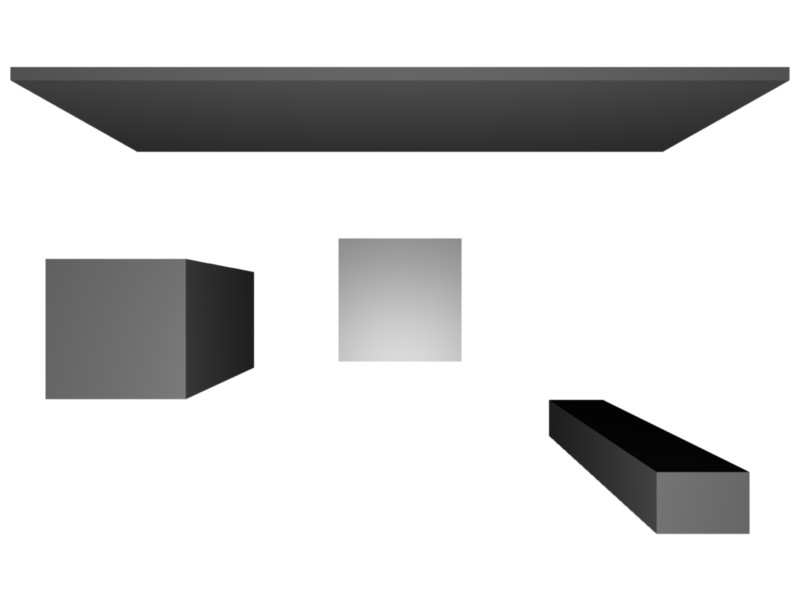
\includegraphics[width=0.5\textwidth]{img/proj_rend.jpg}
%\caption{Rzut perspektywiczny sześcianów}
%\label{fig:proj}
%\end{figure}

\begin{description}
\item[\texttt{Window}] klasa powstała aby zarządzać oknem aplikacji.
\item[\texttt{Options}] tworzy obiekt konfiguracyjny na podstawie pliku i parametrów konsoli.
\item{}
\item[\texttt{GFX::DeferredRenderer}] jedyny moduł odpowiedzialny za rysowanie planet w każdej klatce. Zastąpił on poszczególne klasy, robiąc wszystko sam.
\item[\texttt{GFX::PlanetsTracer}] klasa służąca do zbierania i wyświetlania śladu za planetami. Powstała jako dodatkowa funkcjonalność z ciekawości jak zachowują się planety.
\item[\texttt{GFX::TexturesManager}] klasa przeniesiona z przestrzeni \texttt{FILE2CPU} z powodu wygody użytkowania. Agreguje już załadowane tekstury aby nie ładować tych samych kilka razy. Z uwagi na nowy silnik graficzny, jej użycie jest znikome.
\item[\texttt{GFX::ShaderManager}] analogiczna klasa do \texttt{TextureManager}a, tylko służąca do ładowania shaderów. Powstała po tym, jak niewygodne okazało się ich używanie.
\item[\texttt{GFX::Program}] reprezentuje program OpenGLa składający się z 2 lub 3 shaderów.
\item{}
\item[\texttt{UI::PlanetzPicker}] jest klasą odpowiedzialną za dowiadywanie się która planeta została wciśnięta myszką. Powstała po tym jak uznaliśmy że taka funkcjonalność jest bardzo przydatna.
\item[\texttt{UI::CameraMgr}] zastąpiła dawną klasę \texttt{GFX::Camera}. Dzięki niej możliwa jest zmiana kamer i zarządzanie nimi.
\item[\texttt{UI::Camera}] jest bazową klasą dla wszystkich rodzajów kamer.
\end{description}
\paragraph{}

Podejście deferred renderingu spowodowało również to, że silnik graficzny musi mieć wszystko pod swoją kontrolą. Nie można już założyć że każdy efekt graficzny komunikuje się niezależnie z openglem. Spowodowane jest to niestandardowym podejściem do wyświetlania planet. Dlatego usunięte z struktury programu zostały oddzielne klasy realizujące każdy efekt graficzny, na rzecz jednej klasy wyświetlającej całość planet.

\subsubsection{Wybór}\label{ssub:klikanie}
\paragraph{}

Niestandardowy silnik graficzny spowodował również, że niemożliwe było użycie bezpośrednio opengla do sprawdzania która planeta została kliknięta myszką. Konieczne było napisanie swojego rozwiązania. Bazuje ono mocno na podejściu które można znaleźć w openglu, jednak jest napisane ręcznie.


	\chapter{Raport końcowy}\label{chap:raport końcowy}
	\section{Dokumentacja}\label{sec:dokumentacja}
	\paragraph{}

Dokumentacja została wygenerowana za pomocą programu Doxygen z komentarzy tworzonych podczas pisania kodu. Może być ona dostępna zarówno jako strona html oraz jako dokument w formacie pdf. Jednak z powodu dużych rozmiarów wygenerowanego dokumentu zdecydowaliśmy się na pozostawienie go w formie elektronicznej.


	\section{Raport z testów}\label{sec:raport z testów}
	\subsection{Silnik graficzny}\label{sub:silnik graficzny}

\subsection{Silnik fizyczny}\label{sub:silnik fizyczny}


	\section{Podział pracy}\label{sec:podzial}
	\input{distr.tex}

	\newpage
	\thispagestyle{empty}

\mbox{}
\vspace{0.15\paperheight}

Warszawa, dnia \rule{4cm}{0.5pt}

\vspace{2em}

\begin{center}
{\large Oświadczenie}
\end{center}

\vspace{1em}

Oświadczam, że moją część pracy inżynierskiej (zgodnie z podziałem zadań opisanym w~sekcji \ref{sec:podzial}) pod tytułem ,,Symulacja układu planetarnego na GPU przy użyciu CUDA i OpenGL'', której promotorem jest dr~inż. Krzysztof Kaczmarski, wykonałem samodzielnie, co poświadczam własnoręcznym podpisem.

\vspace{3em}

\hfill\rule{5cm}{0.5pt}

	\newpage

\end{document}

